%0       1         2         3         4         5         6         7         8
%2345678901234567890123456789012345678901234567890123456789012345678901234567890

\documentclass[10pt]{article}


% INCLUDE DEVELOPMENT TEXT

\newcommand{\devel}[1]{\textbf{#1}}

% EXCLUDE DEVELOPMENT TEXT

% \newcommand{\devel}[1]{}


%=======================================================================
% Document layout
%=======================================================================

\setlength{\topmargin}{0.0in}
\setlength{\oddsidemargin}{0.0in}
\setlength{\evensidemargin}{0.0in}
\setlength{\textwidth}{6.0in}
\setlength{\textheight}{9.0in}

%=======================================================================
% Packages
%=======================================================================

\usepackage{wasysym}
\usepackage{epsfig}
\usepackage{url}

%=======================================================================
% Commands
%=======================================================================

\newcommand{\cello}{\textsf{Cello}}
\newcommand{\enzo}{\textsf{Enzo}}
\newcommand{\lcaperf}{\textsf{lcaperf}}
\newcommand{\lcatest}{\textsf{lcatest}}

\newcommand{\code}[1]{\textsf{#1}}

\newcommand{\note}[1]{\devel{\eighthnote\ \textit{#1} \\}}
\newcommand{\pargraph}[1]{\devel{\P\ \textbf{#1} \\}}

\newcommand{\todo}{\devel{$\circ$}}
\newcommand{\done}{\devel{$\bullet$}}
\newcommand{\halfdone}{\devel{\textcolor{gray}{$\bullet$}}}

\newcommand{\PROJECT}{\cello}

\newcommand{\TITLE}[3]{
\title{ {\huge \PROJECT\ #1}  \\ \vspace{0.1in}
     {\small Document Version: \textbf{#3}} \vspace{-0.1in}
    }
\author{      #2 \\
        Laboratory for Computational Astrophysics\\
        University of California, San Diego}
\maketitle}

%=======================================================================


%==================================================================
% Margins and spacing
%==================================================================

\begin{document}

%=======================================================================
\TITLE{\hypre\ SAMR Linear Solver}
      {James Bordner}
      {in preparation}
%=======================================================================

\tableofcontents
%======================================================================
\section{Overview}
%======================================================================

   \hypresolve\ will be used as a testbed for experimenting with the
   parallel solution of linear systems arising from self-gravity and
   radiation transfer algorithms defined on distributed SAMR
   hierarchies.  The purpose of this document is to specify the
   requirements, describe the design and implementation, and present
   test results for \hypresolve.

   We break the problem into two phases: problem generation
   (\code{hypre-init}), and problem solution (\code{hypre-solve}).
   \code{hypre-init} takes as input parameters describing the problem
   characteristics in general terms, such as bounds on grid sizes,
   number of processors, description of how to distribute point
   masses, etc.  The output is a file of parameters that specify the
   exact problem to solve, including grid locations, sizes, levels,
   point mass locations, etc.  This file output by \code{hypre-init}
   is subsequently input by \code{hypre-solve}, together with
   solver-specific parameters.  A distributed linear system is
   assembled and solved using \hypre, and the solution, performance
   information, solver efficiency information, etc., are output.

   \note{top-level diagram: problem description $\Rightarrow$
   \code{hypre-init} $\Rightarrow$ problem specification $\Rightarrow$
   \code{hypre-solve} $\Rightarrow$ problem results}

%======================================================================
\section{Components}
%======================================================================

%-----------------------------------------------------------------------
\subsection{\code{hypre-init}} \label{ss:hypre-init}
%-----------------------------------------------------------------------

\subsubsection{Input}  \label{sss:hypre-init-input}

\begin{tabbing}
xxxxx\=xxxxxxxxxxxxxxxxxxxxxxxx\=\kill
\> \todo\ \code{dimension} \> \code{\textit{int dimension}} \\
\> \todo\ \code{particle\_position\_clumpiness}  \\
\> \todo\ \code{particle\_mass\_clumpiness} \\
\> \todo\ \code{particle\_mass\_average} \\
\> \todo\ \code{sphere} \> \code{\textit{Scalar mass}, \textit{Scalar radius}, \textit{Scalar 3*center}} \\
\> \todo\  \code{domain\_extents} \\
\> \todo\  \code{processor\_grid} \\
\> \todo\ \code{discret} \> \code{\textit{int type}} \\
\> \todo\  \code{levels} \\
\> \todo\ \code{solver} \> \code{\{"fac"\} method}
\end{tabbing}

\subsubsection{Output} \label{sss:hypre-init-output}

See \S\ref{sss:hypre-solve-input}.


% \textbf{Input}
% 
% \begin{tabbing}
% xxxxx\=xxx\=\kill\\ 
% \> \todo \>  Maximum number of point masses \\
% \> \todo \>  Description of probability distribution of point masses \\
% \> \todo \>  Number of spheres \\
% \> \todo \>  Positions of spheres \\
% \> \todo \>  Masses of spheres \\
% \> \todo \>  Extents of the domain \\
%  \\
% \> \todo \>  Lower bound on grid sizes \\
% \> \todo \>  Upper bound on grid sizes \\
% \> \todo \>  Upper bound on number of grids \\
%  \\
% \> \todo \>  AMR hierarchy depth \\
% \> \todo \>  AMR Refinement factor (2,3,4) \\
% \end{tabbing}
% 
% \textbf{Output}
% 
%  depth of refinement point layer around point masses
%  depth of refinement point layer around spheres


%-----------------------------------------------------------------------
\subsection{\code{hypre-solve}}  \label{ss:hypre-solve}
%-----------------------------------------------------------------------

\subsubsection{Input} \label{sss:hypre-solve-input}

The following table lists the input parameters to \code{hypre-solve}.

\begin{tabbing}
xxxxx\=xxxxxxxxxxx\=\kill
\> \done\ \code{dimension} \> \code{\textit{int dimension}} \\
\> \done\ \code{sphere} \> \code{\textit{Scalar mass}, \textit{Scalar radius}, \textit{Scalar 3*center}} \\
\> \done\ \code{point} \> \code{\textit{Scalar mass}, \textit{Scalar 3*location}} \\
\> \todo\ \code{grid} \> \code{\textit{int id}, \textit{int parent-id}, \textit{int processor}, \textit{Scalar vertex-lower}, \textit{Scalar vertex-upper}, \textit{int 3*zones}} \\
\> \todo\ \code{discret} \> \code{\textit{int type}} \\
\> \todo\ \code{solver} \> \code{\{"fac"\} method}
\end{tabbing}


\subsubsection{Output}  \label{sss:hypre-solve-output}

\begin{tabbing}
xxxxx\=xxxxxxxxxxxxxx\=\kill
\> \todo\ \code{flops-balance} \>    \textit{Load balance efficiency with respect to flops}\\
\> \todo\ \code{flops-proc-avg} \> \textit{Average flop counts over processors} \\
\> \todo\ \code{flops-proc-max} \> \textit{Maximum flop counts over processors} \\
\> \todo\ \code{flops-total} \> \textit{Number of floating point operations} \\
\> \todo\ \code{mem-balance} \>    \textit{Load balance efficiency with respect to memory}\\
\> \todo\ \code{mem-proc-avg} \> \textit{Average memory usage over processors} \\
\> \todo\ \code{mem-proc-max} \>    \textit{Maximum memory usage over processors} \\
\> \todo\ \code{mem-total} \> \textit{Amount of memory used} \\
\> \todo\ \code{procs-total} \> \textit{Number of processors} \\
\> \todo\ \code{time-total} \>  \textit{Time to solution}
\end{tabbing}


%======================================================================
\section{Using \hypre}
%======================================================================

This section describes the sequence of calls in \hypre\ used for
setting up a linear system on an AMR hierarchy, and then solving it.

\begin{enumerate}
\item Initialize \hypre\ grids (\S\ref{ss:hypre-grids})
\item Initialize \hypre\ stencil (\S\ref{ss:hypre-stencil})
\item Initialize \hypre\ graph (\S\ref{ss:hypre-graph})
\item Initialize \hypre\ matrix (\S\ref{ss:hypre-matrix})
\item Initialize \hypre\ vectors (\S\ref{ss:hypre-vectors})
\end{enumerate}

%-----------------------------------------------------------------------
\subsection{Initialize \hypre\ grids} \label{ss:hypre-grids}
%-----------------------------------------------------------------------

For each grid patch it owns, each processor creates a \hypre\ grid
object defining the grid's extents and variables.

\begin{itemize}
\item \code{HYPRE\_SStructGridCreate()}
\item \code{HYPRE\_SStructGridSetExtents()}
\item \code{HYPRE\_SStructGridSetVariables()}
\item \code{HYPRE\_SStructGridAssemble()}
\end{itemize}

%-----------------------------------------------------------------------
\subsection{Initialize \hypre\ stencil} \label{ss:hypre-stencil}
%-----------------------------------------------------------------------

  Create the stencil object which defines the matrix nonzeros within each grid.

\begin{itemize}
\item \code{HYPRE\_SStructStencilCreate()}
\item \code{HYPRE\_SStructStencilSetEntry()}
\end{itemize}

%-----------------------------------------------------------------------
\subsection{Initialize \hypre\ graph} \label{ss:hypre-graph}
%-----------------------------------------------------------------------

 Each processor creates a graph containing the nonzero structure of
 the matrix.

\begin{itemize}
\item \code{HYPRE\_SStructGraphCreate()}
\item \code{HYPRE\_SStructGraphSetStencil()}
\item \code{HYPRE\_SStructGraphAddEntries()}
\item \code{HYPRE\_SStructGraphAssemble()}
\end{itemize}

%-----------------------------------------------------------------------
\subsection{Initialize \hypre\ matrix} \label{ss:hypre-matrix}
%-----------------------------------------------------------------------

\begin{itemize}
\item \code{HYPRE\_SStructMatrixCreate()}
\item \code{HYPRE\_SStructMatrixInitialize()}
\item \code{HYPRE\_SStructMatrixSetBoxValues()}
\item \code{HYPRE\_SStructMatrixSetValues()}
\item \code{HYPRE\_SStructMatrixAssemble()}
\end{itemize}

%-----------------------------------------------------------------------
\subsection{Initialize \hypre\ vectors} \label{ss:hypre-vectors}
%-----------------------------------------------------------------------

\begin{itemize}
\item \code{HYPRE\_SStructVectorCreate()}
\item \code{HYPRE\_SStructVectorInitialize()}
\item \code{HYPRE\_SStructVectorSetBoxValues()}
\item \code{HYPRE\_SStructVectorAssemble()}
\end{itemize}

%=======================================================================
\section{Design} \label{s:design}
%=======================================================================

%-----------------------------------------------------------------------
\section{Classes} \label{ss:classes}
%-----------------------------------------------------------------------

%-----------------------------------------------------------------------
\subsection{AMR classes}

The AMR hierarchy is represented using the trio of classes
\code{hierarchy}, \code{Level}, and \code{Grid}.  A \code{Grid} is a
box in space, and is decomposed into \code{GridLocal} and
\code{GridRemote} classes (see \S\ref{sss:class-grid}).  Each
\code{GridLocal} object has some number of \code{Field} objects
associated with them (see \S\ref{sss:class-field}), though the
\code{GridLocal} objects themselves do not store field data
themselves.  A \code{Level} class is also either a ``structured''
\code{LevelStruct} or an ``unstructured'' \code{LevelUnstruct}.
Structured levels are composed of a regular array of \code{Grid}s, and
is typically used for unigrid calculations or the root level of an AMR
calculation.  Unstructured levels are typically used for non-root
levels of an AMR calulation.

\begin{center}
\epsfig{file=uml/hierarchy.1,width=0.75in}
\end{center}

%-----------------------------------------------------------------------
\subsubsection{\code{Hierarchy} class} \label{sss:class-hierarchy}

\begin{center}
\epsfig{file=uml/class-hierarchy.1,width=1.5in}
\end{center}

%-----------------------------------------------------------------------
\subsubsection{\code{Level} class} \label{sss:class-level}

\begin{center}
\epsfig{file=uml/class-level.1,width=1.5in}
\end{center}

%-----------------------------------------------------------------------
\subsubsection{\code{Grid} class} \label{sss:class-grid}

\begin{center}
\epsfig{file=uml/grid.1,     width=2.00in}
\end{center}


\begin{center}
\epsfig{file=uml/class-grid.1,width=2.5in}
\end{center}

%-----------------------------------------------------------------------
\subsection{Problem classes}

\code{Problem}, \code{Sphere}, and \code{Point}

%-----------------------------------------------------------------------
\subsubsection{\code{Problem} class} \label{sss:class-problem}

\begin{center}
\epsfig{file=uml/class-problem.1,width=2.0in}
\end{center}

%-----------------------------------------------------------------------
\subsubsection{\code{Sphere} class} \label{sss:class-sphere}

\begin{center}
\epsfig{file=uml/class-sphere.1,width=1.0in}
\end{center}

%-----------------------------------------------------------------------
\subsection{Discretization classes}

%-----------------------------------------------------------------------
\subsubsection{\code{Discret} class} \label{sss:class-discret}

\begin{center}
\epsfig{file=uml/class-discret.1,width=2.5in}
\end{center}

%-----------------------------------------------------------------------
\subsubsection{\code{Hypre} class}  \label{sss:class-hypre}

\begin{center}
\epsfig{file=uml/class-hypre.1,width=2.0in}
\end{center}

%-----------------------------------------------------------------------
\subsubsection{\code{Mpi} class} \label{sss:class-mpi}

\begin{center}
\epsfig{file=uml/class-mpi.1,width=1.5in}
\end{center}

%-----------------------------------------------------------------------
\subsubsection{\code{Point} class} \label{sss:class-point}

\begin{center}
\epsfig{file=uml/class-point.1,width=1.0in}
\end{center}

%-----------------------------------------------------------------------
\subsubsection{\code{Field} class} \label{sss:class-field}

\begin{center}
\epsfig{file=uml/field.1,     width=0.75in}
\end{center}

%-----------------------------------------------------------------------
\subsubsection{\code{Array} class} \label{sss:class-array}

%=======================================================================
\section{Discretization} \label{s:discretization}
%=======================================================================

\newcommand{\indvar}{r}
 \newcommand{\uc}{u(\indvar)}

 \newcommand{\uxp}{u(\indvar+h_x)}
 \newcommand{\uxm}{u(\indvar-h_x)}
 \newcommand{\uxph}{u(\indvar+\frac{h_x}{2})}
 \newcommand{\uxmh}{u(\indvar-\frac{h_x}{2})}

 \newcommand{\uyp}{u(\indvar+h_y)}
 \newcommand{\uym}{u(\indvar-h_y)}
 \newcommand{\uyph}{u(\indvar+\frac{h_y}{2})}
 \newcommand{\uymh}{u(\indvar-\frac{h_y}{2})}

 \newcommand{\uzp}{u(\indvar+h_z)}
 \newcommand{\uzm}{u(\indvar-h_z)}
 \newcommand{\uzph}{u(\indvar+\frac{h_z}{2})}
 \newcommand{\uzmh}{u(\indvar-\frac{h_z}{2})}

 \newcommand{\ac}{a(\indvar)}
 \newcommand{\axph}{a(\indvar+\frac{h_x}{2})}
 \newcommand{\axmh}{a(\indvar-\frac{h_x}{2})}
 \newcommand{\ayph}{a(\indvar+\frac{h_y}{2})}
 \newcommand{\aymh}{a(\indvar-\frac{h_y}{2})}
 \newcommand{\azph}{a(\indvar+\frac{h_z}{2})}
 \newcommand{\azmh}{a(\indvar-\frac{h_z}{2})}

 \newcommand{\alc}{\alpha_{0}}
 \newcommand{\alxp}{\alpha_{x}}
 \newcommand{\alxm}{\alpha_{\bar{x}}}
 \newcommand{\alyp}{\alpha_{y}}
 \newcommand{\alym}{\alpha_{\bar{y}}}
 \newcommand{\alzp}{\alpha_{z}}
 \newcommand{\alzm}{\alpha_{\bar{z}}}

 \newcommand{\Uc}{U_{0}}
 \newcommand{\Uxp}{U_{x}}
 \newcommand{\Uxm}{U_{\bar{x}}}
 \newcommand{\Uyp}{U_{y}}
 \newcommand{\Uym}{U_{\bar{y}}}
 \newcommand{\Uzp}{U_{z}}
 \newcommand{\Uzm}{U_{\bar{z}}}

%-----------------------------------------------------------------------
\subsection{Discretization within levels}
%-----------------------------------------------------------------------

We assume that grid spacing $h_x$, $h_y$, and $h_z$ within a level is uniform.

\begin{center}
\begin{minipage}{1.5in}
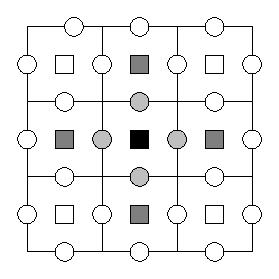
\epsfig{file=fig/stencil.eps,width=1.5in}
\end{minipage} \[ \nabla\cdot(\ac \nabla \uc) = \bar{\rho} \]
\end{center}


 \begin{eqnarray*}
 \nabla\cdot(\ac \nabla \uc) & = & D_x (\ac D_x \uc) + D_y (\ac D_y \uc) + D_z (\ac D_z \uc) \\
 & \approx & \frac{\delta_{h_x}}{h_x} (\ac \frac{\delta_{h_x}}{h_x} \uc) + 
             \frac{\delta_{h_y}}{h_y} (\ac \frac{\delta_{h_y}}{h_y} \uc) + 
             \frac{\delta_{h_z}}{h_z} (\ac \frac{\delta_{h_z}}{h_z} \uc) \\
% & \approx & \frac{1}{h_x^2}\delta_{h_x} (\ac \delta_{h_x} \uc) + 
%             \frac{1}{h_y^2}\delta_{h_y} (\ac \delta_{h_y} \uc) + 
%             \frac{1}{h_z^2}\delta_{h_z} (\ac \delta_{h_z} \uc) \\
% & = & \frac{1}{h_x^2}\delta_{h_x} (\ac (\uxph - \uxmh))\\
% & + & \frac{1}{h_y^2}\delta_{h_y} (\ac (\uyph - \uymh)) \\
% & + & \frac{1}{h_z^2}\delta_{h_z} (\ac (\uzph - \uzmh)) \\
% & = & \frac{1}{h_x^2} (\axph (\uxp - \uc)) - (\axmh (\uc - \uxm)) \\
% & + & \frac{1}{h_y^2} (\ayph (\uyp - \uc)) - (\aymh (\uc - \uym)) \\
% & + & \frac{1}{h_z^2} (\azph (\uzp - \uc)) - (\azmh (\uc - \uzm)) \\
% & = & \frac{1}{h_z^2} \azmh \uzm + \frac{1}{h_y^2} \aymh \uym + \frac{1}{h_x^2} \axmh \uxm \\
% & - & [\frac{1}{h_x^2} \axph  + \frac{1}{h_x^2} \axmh \\
% & &+  \frac{1}{h_y^2} \ayph  + \frac{1}{h_y^2} \aymh \\
% & & +  \frac{1}{h_z^2} \azph  + \frac{1}{h_z^2} \azmh] \uc \\
% & + &  \frac{1}{h_x^2} \axph \uxp + \frac{1}{h_y^2} \ayph \uyp  + \frac{1}{h_z^2} \azph \uzp \\
 & \approx & \alzm\Uzm +  \alym\Uym +  \alxm\Uxm 
  +  \alc\Uc 
  +  \alxp\Uxp +  \alyp\Uyp +  \alzp\Uzp,
 \end{eqnarray*}
where

\[\alxm  \equiv  \frac{1}{h_x^2} \axmh,
 \alym  \equiv  \frac{1}{h_y^2} \aymh, 
 \alzm  \equiv  \frac{1}{h_z^2} \azmh \]
 \[\alxp  \equiv  \frac{1}{h_x^2} \axph, 
 \alyp  \equiv  \frac{1}{h_y^2} \ayph,
 \alzp  \equiv  \frac{1}{h_z^2} \azph \]
 \[\alc   \equiv  - [\alxm + \alym + \alzm + \alxp + \alyp + \alzp] \]

%-----------------------------------------------------------------------
\subsection{Discretization between levels}
%-----------------------------------------------------------------------

We assume that grid spacing ($h^i_x$, $h^i_y$, $h^i_z$) and 
($h^j_x$, $h^j_y$, $h^j_z$) between levels $i < j$ is such that
$h^j_* / h^i_*$ is an integer.


\subsubsection{$h^j_* / h^i_* = 2$}


\begin{center}
\begin{minipage}{1.25in}
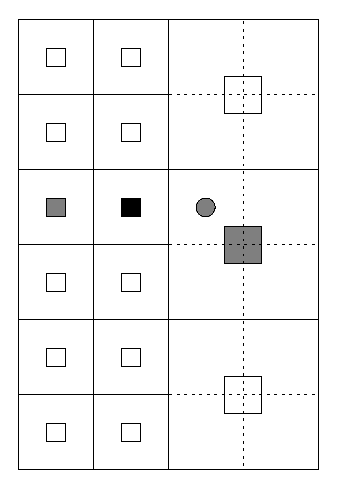
\epsfig{file=fig/stencil0.eps,width=1.25in}
\end{minipage} \ \ \ 
\begin{minipage}{1.25in}
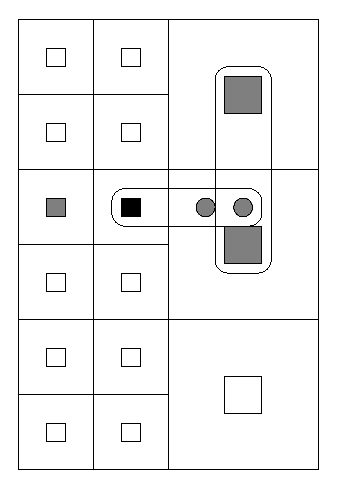
\epsfig{file=fig/stencil1.eps,width=1.25in}
\end{minipage} \ \ \ 
\begin{minipage}{1.25in}
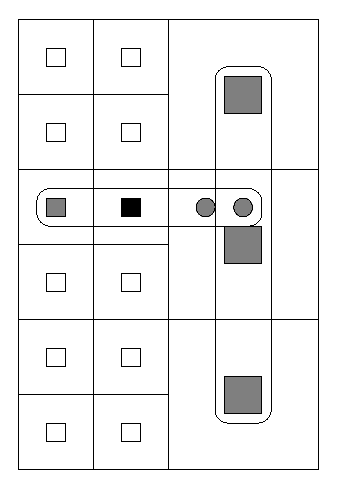
\epsfig{file=fig/stencil2.eps,width=1.25in}
\end{minipage}
\end{center}



\begin{center}
\begin{minipage}{2in}
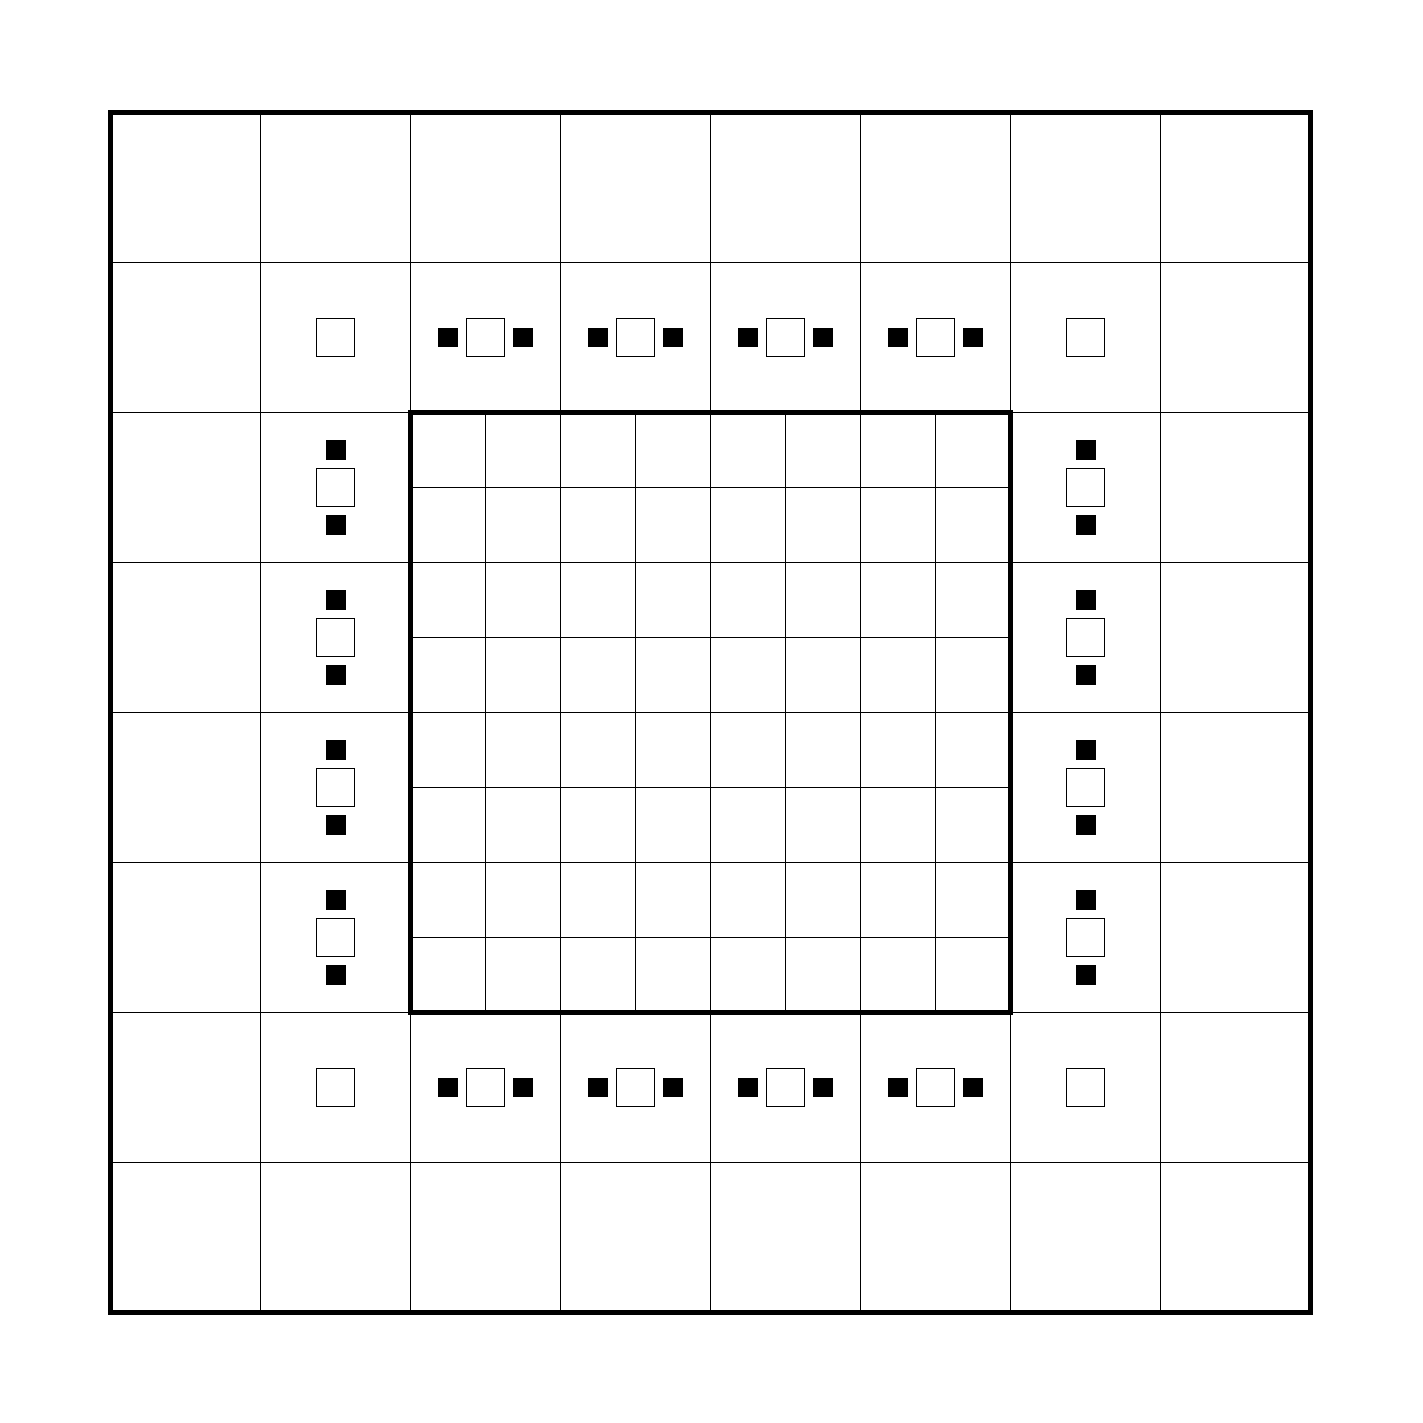
\epsfig{file=fig/discret6.eps,width=2.0in}
\end{minipage}$\Rightarrow$
\begin{minipage}{2in}
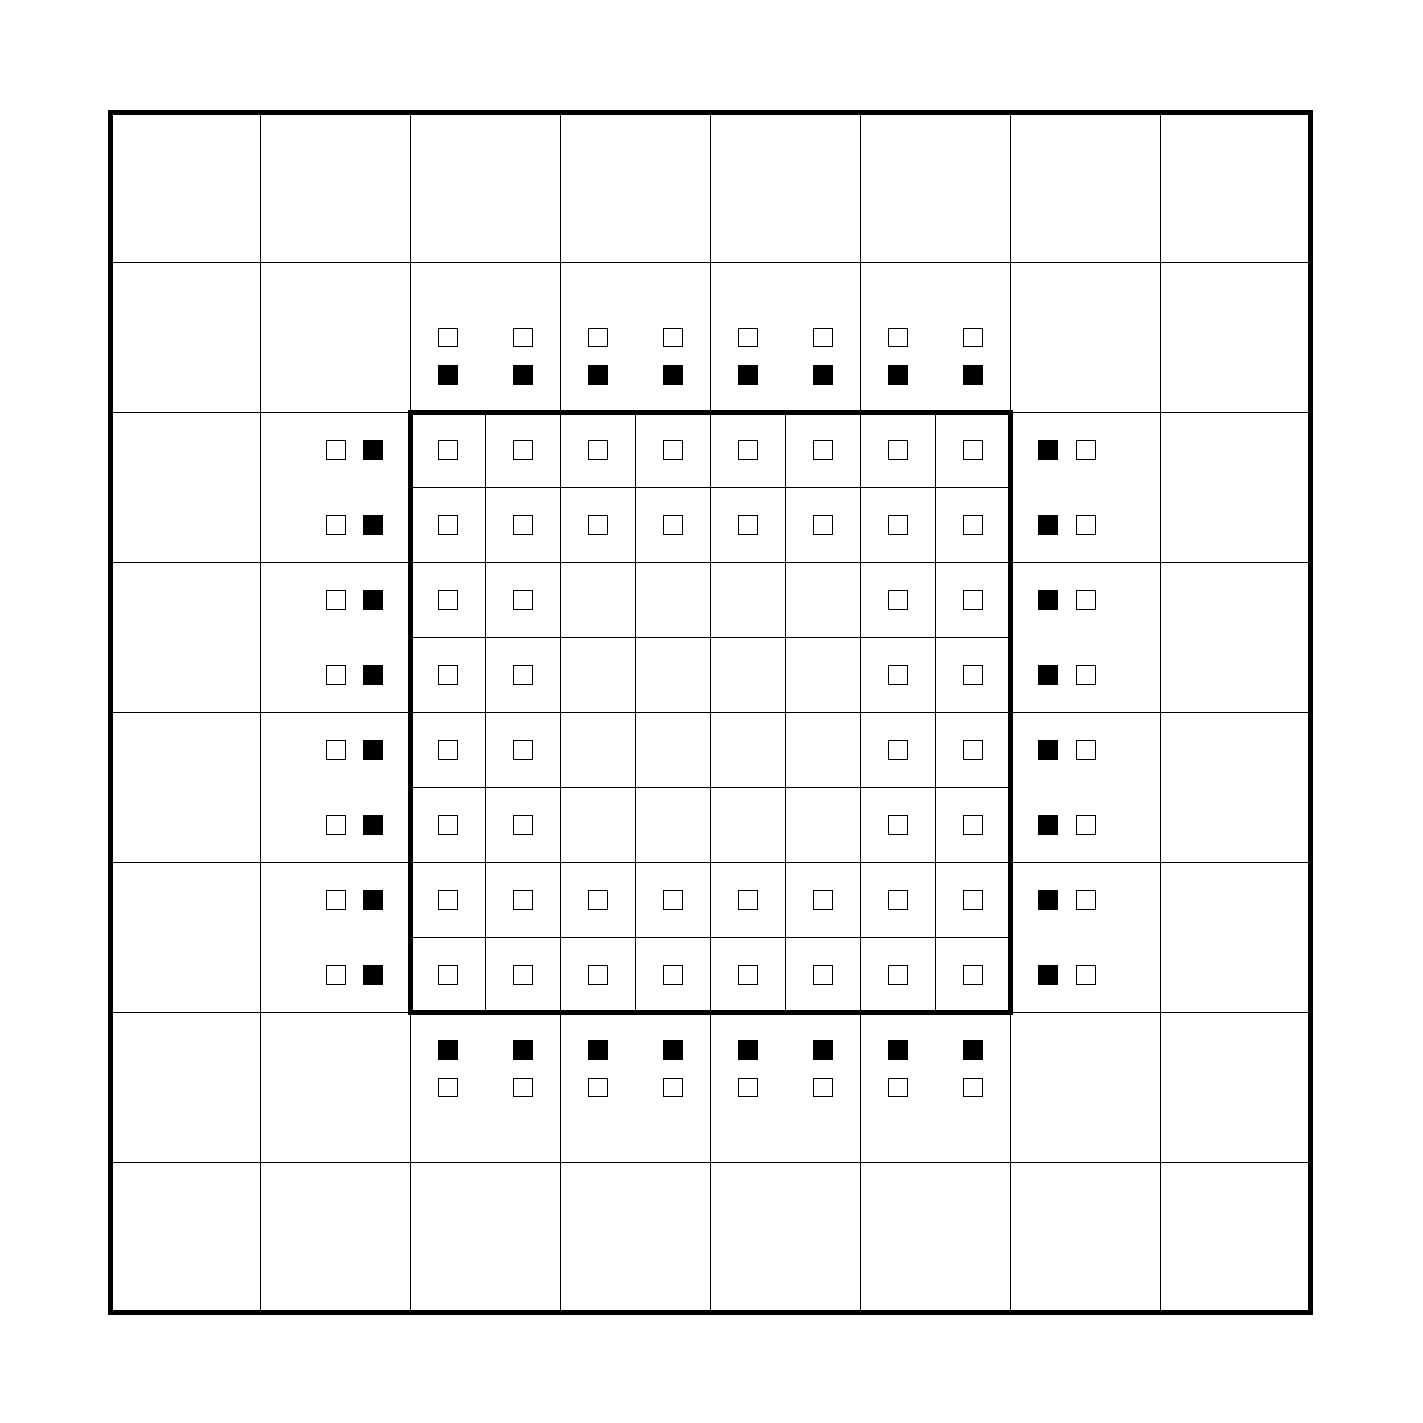
\epsfig{file=fig/discret5.eps,width=2.0in}
\end{minipage}$\Rightarrow$
\begin{minipage}{2in}
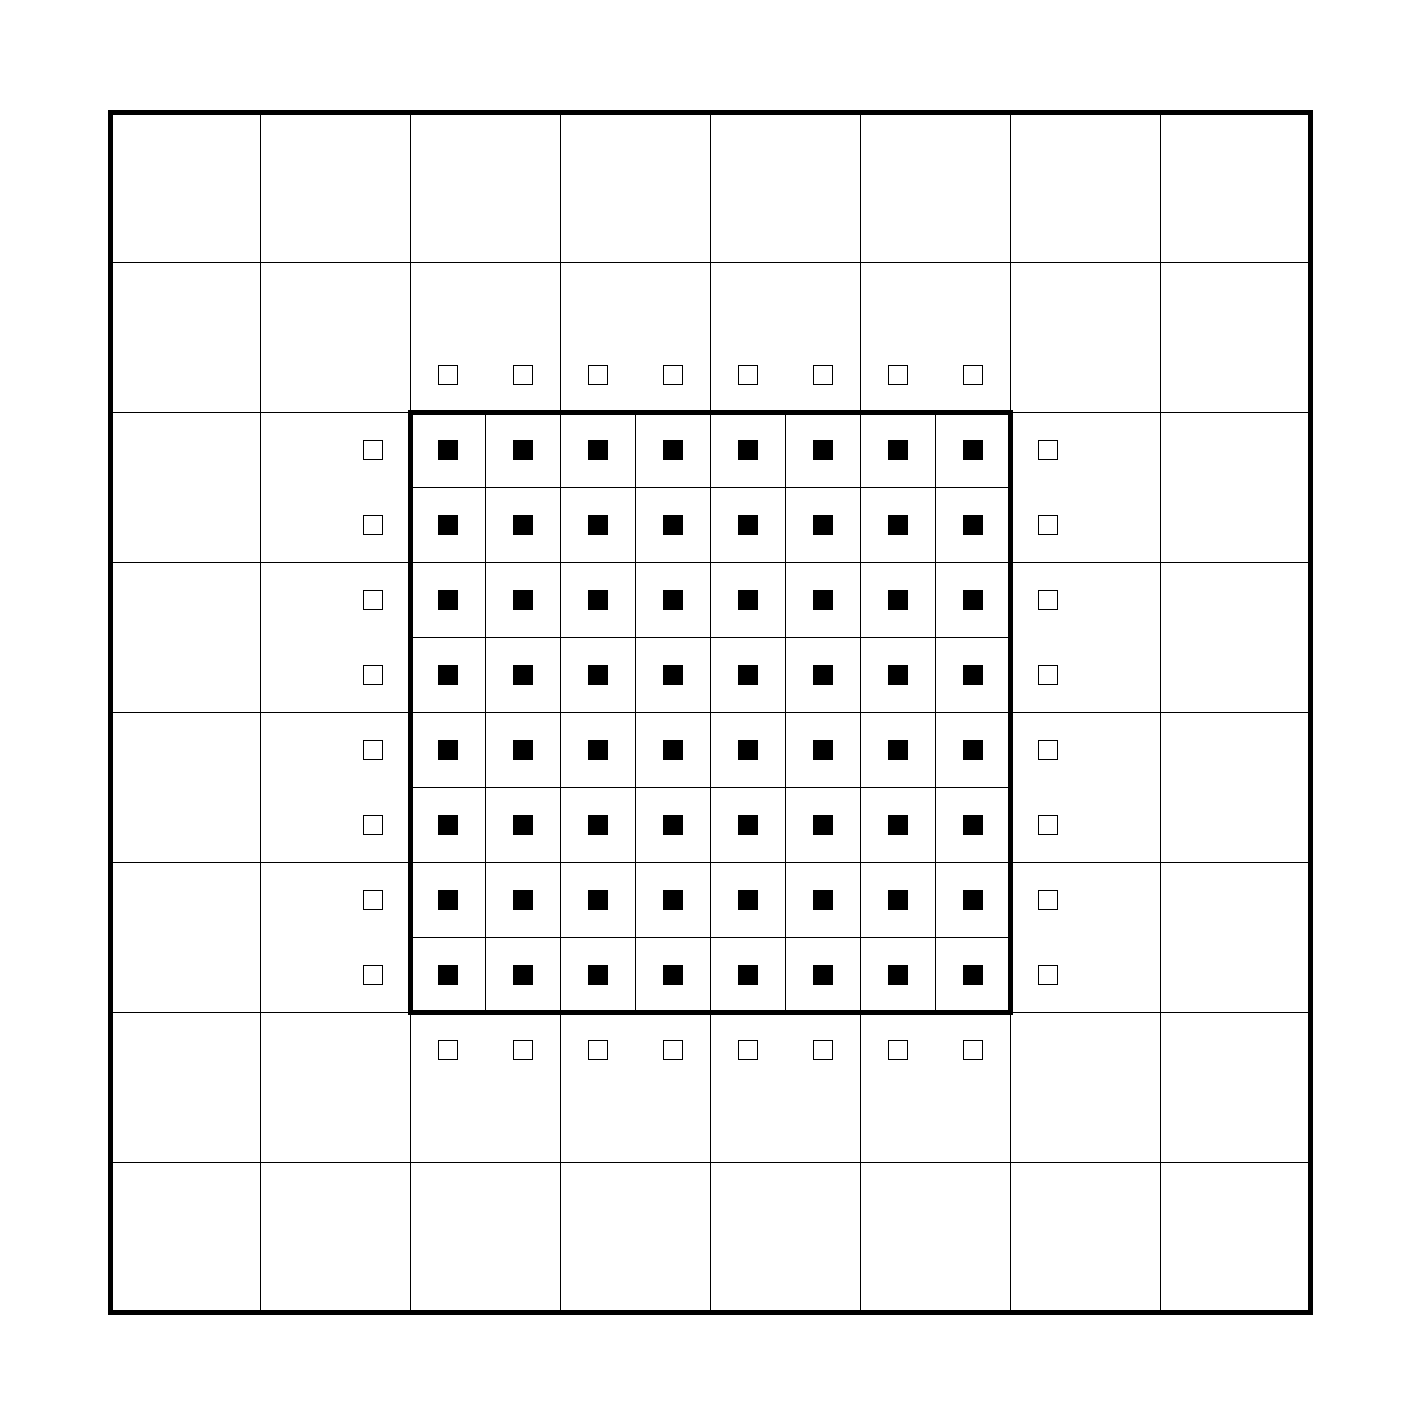
\epsfig{file=fig/discret4.eps,width=2.0in}
\end{minipage} \\
\begin{minipage}{4.5in}
\hfill $\Downarrow$
\end{minipage} \\
\begin{minipage}{2in}
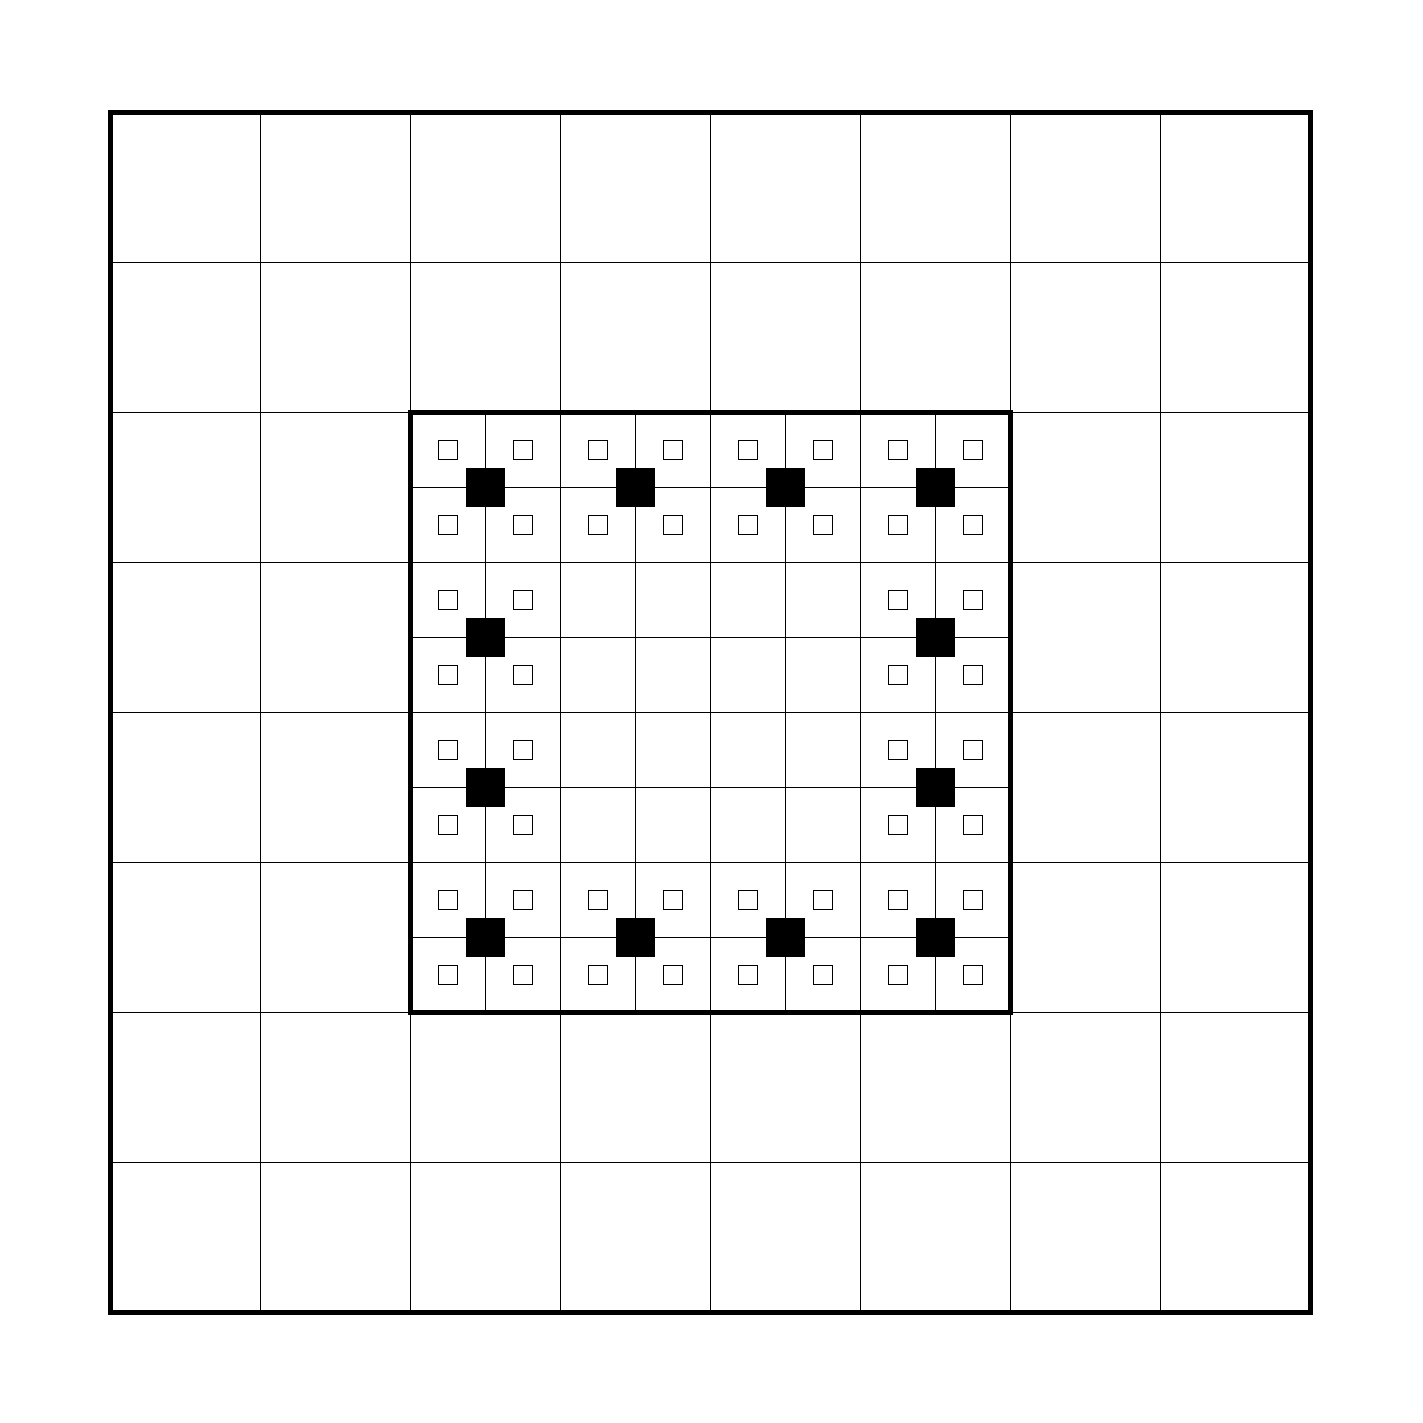
\epsfig{file=fig/discret3.eps,width=2.0in}
\end{minipage}$\Rightarrow$
\begin{minipage}{2in}
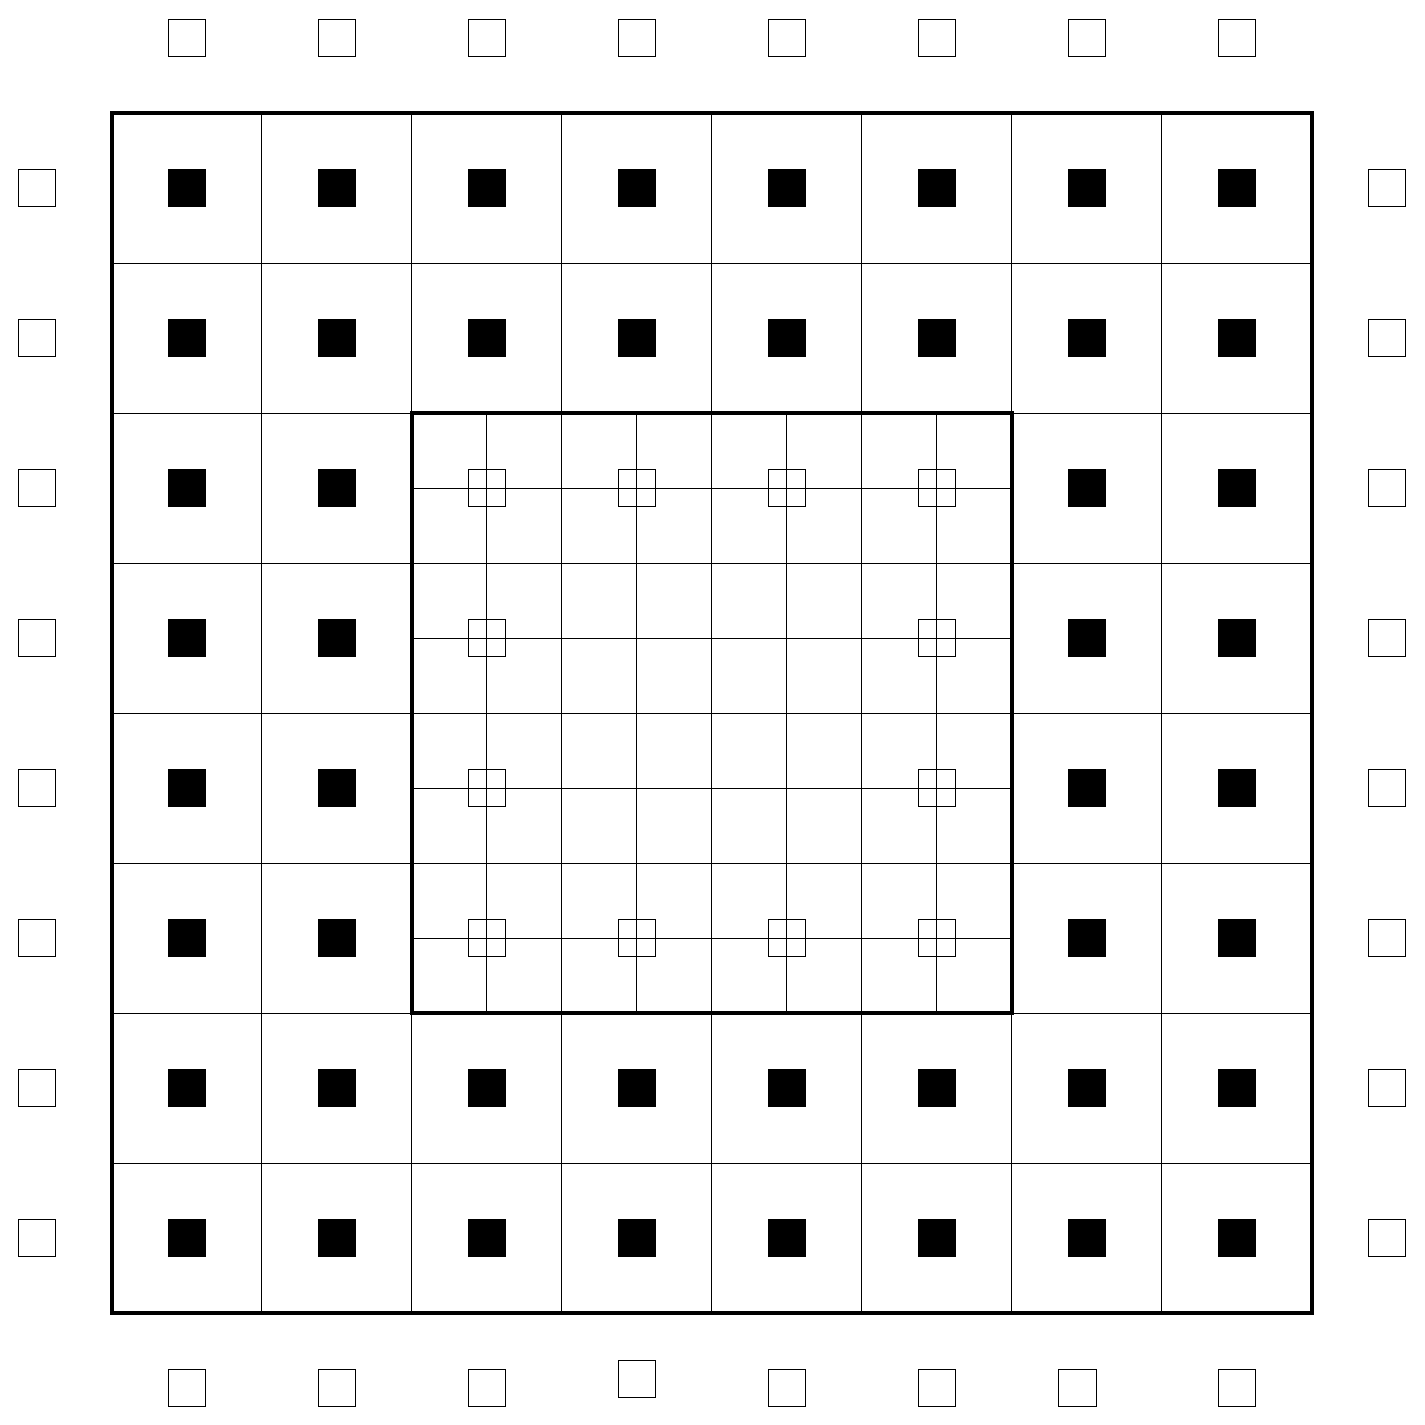
\epsfig{file=fig/discret2.eps,width=2.0in}
\end{minipage}$\Rightarrow$
\begin{minipage}{2in}
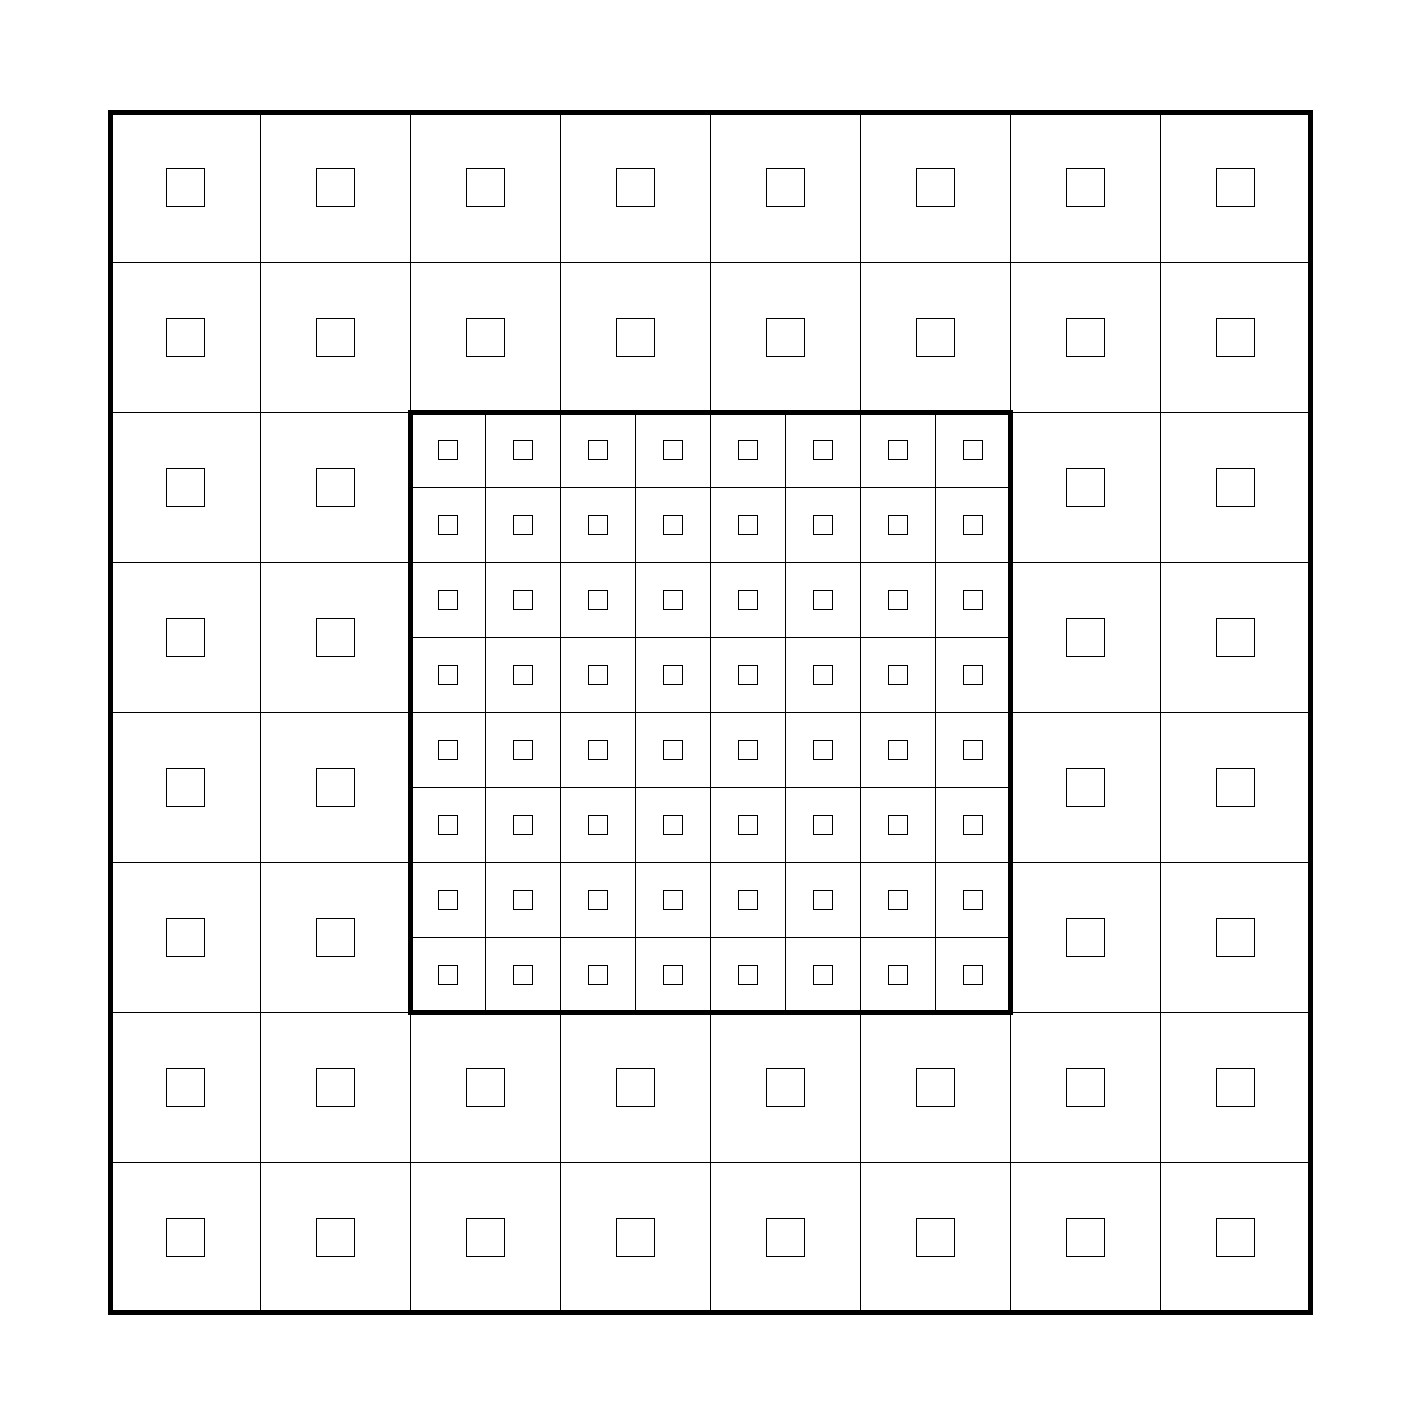
\epsfig{file=fig/discret1.eps,width=2.0in}
\end{minipage}
\end{center}

\begin{center}
\begin{minipage}{6.0in}
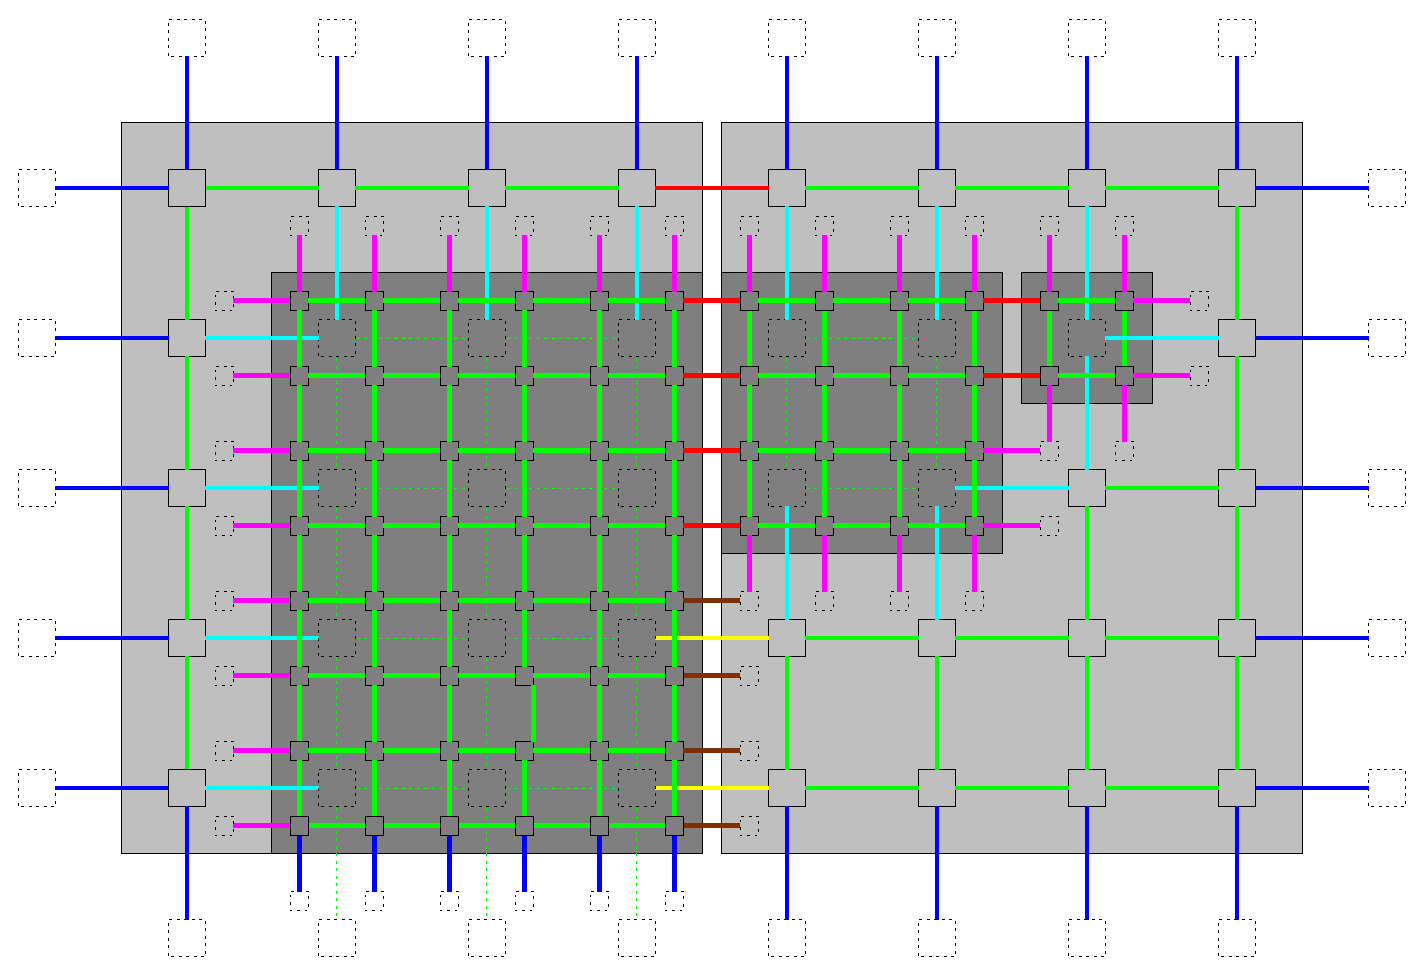
\epsfig{file=fig/discret-step-1.eps,width=6.0in}
\end{minipage}
\end{center}

Grid patches are controlled using
\begin{itemize}
\item \code{HYPRE\_SStructGridCreate()}
\item \code{HYPRE\_SStructGridSetExtents()}
\item \code{HYPRE\_SStructGridSetVariables()}
\item \code{HYPRE\_SStructGridSetNeighborBox()}
\item \code{HYPRE\_SStructGridAssemble()}
\item \code{HYPRE\_SStructGridSetNumGhost()}
\item \code{HYPRE\_SStructGridDestroy()}
\end{itemize}

Stencils are controlled using
\begin{itemize}
\item \code{HYPRE\_SStructStencilCreate()}
\item \code{HYPRE\_SStructStencilSetEntry()}
\item \code{HYPRE\_SStructStencilDestroy()}
\end{itemize}

Graphs are controlled using
\begin{itemize}
\item \code{HYPRE\_SStructGraphCreate()}
\item \code{HYPRE\_SStructGraphSetStencil()}
\item \code{HYPRE\_SStructGraphAddEntry()}
\item \code{HYPRE\_SStructGraphSetObjectType()}
\item \code{HYPRE\_SStructGraphAssemble()}
\item \code{HYPRE\_SStructGraphDestroy()}
\end{itemize}

Matrices are controlled using
\begin{itemize}
\item \code{HYPRE\_SStructMatrixCreate()}
\item \code{HYPRE\_SStructMatrixInitialize()}
\item \code{HYPRE\_SStructMatrixGetObject()}
\item \code{HYPRE\_SStructMatrixSetObjectType()}
\item \code{HYPRE\_SStructMatrixSetValues()}
\item \code{HYPRE\_SStructMatrixAddToValues()}
\item \code{HYPRE\_SStructMatrixSetBoxValues()}
\item \code{HYPRE\_SStructMatrixAddToBoxValues()}
\item \code{HYPRE\_SStructMatrixDestroy()}
\item \code{HYPRE\_SStructMatrixPrint()}
\end{itemize}

Vectors are controlled using:
\begin{itemize}
\item \code{HYPRE\_SStructVectorCreate()}
\item \code{HYPRE\_SStructVectorInitialize()}
\item \code{HYPRE\_SStructVectorGetObject()}
\item \code{HYPRE\_SStructVectorSetObjectType()}
\item \code{HYPRE\_SStructVectorSetValues()}
\item \code{HYPRE\_SStructVectorAddToValues()}
\item \code{HYPRE\_SStructVectorSetBoxValues()}
\item \code{HYPRE\_SStructVectorAddToBoxValues()}
\item \code{HYPRE\_SStructVectorDestroy()}
\item \code{HYPRE\_SStructVectorPrint()}
\end{itemize}




Types of matrix elements for a given unknown:

\begin{tabular}{ll}
\textcolor{green}{internal} & \code{HYPRE\_SStructStencilSetEntry()} \\
\textcolor{green}{overlapped internal} & \code{HYPRE\_SStructStencil} \\
\textcolor{red}{neighbor} & \code{HYPRE\_SStructGridSetNeighborBox()}\\
\textcolor{blue}{boundary} & \code{HYPRE\_SStructGraphAddEntries()}\\
\textcolor{magenta}{fine-coarse parent} & \code{HYPRE\_SStructGraphAddEntries()}\\
\textcolor{cyan}{coarse-fine child} & \code{HYPRE\_SStructGraphAddEntries()}\\
\textcolor{brown}{fine-coarse parent--neighbor} & \code{HYPRE\_SStructGraphAddEntries()}\\
\textcolor{yellow}{coarse-fine neighbor--child} & \code{HYPRE\_SStructGraphAddEntries()}\\
\end{tabular}

%=======================================================================
\section{Results} \label{s:results}
%=======================================================================

\EndDOCUMENT

\end{document}
%==================================================================

